% define o tipo de documento, isso interfere na organização das seções
\documentclass{article}

% pacote de função para trocar automaticamente caracteres acentuados peplo código correspondente (\'a = á)
\usepackage[utf8]{inputenc}

% pacote de função para gerar o PDF com acentuação
\usepackage[T1]{fontenc}

% pacote para identar o primeiro parágrado
\usepackage{indentfirst}

% informar para o compilador que o documento é em pt-BR
\usepackage[brazil]{babel}

% mudar as margens
\usepackage[top=2cm, left=2cm, right=1cm, bottom=3cm]{geometry}

% funções de manipulação de imagens
\usepackage{graphicx}

\begin{document}

\tableofcontents
\newpage % se o documentclass for book ele já quebra página

\section{Introdução}
Meu primeiro texto utilizando látex. É um teste simples.

\section{Método}

Lorem ipsum..Lorem ipsum..Lorem ipsum..Lorem ipsum..Lorem ipsum..Lorem ipsum..Lorem ipsum..\\ %quebra de linha
Lorem ipsum..Lorem ipsum.. Lorem ipsum..Lorem ipsum..Lorem ipsum..
\subsection{Objetivos}
Aqui teremos os nosso objetivos. Aqui teremos os nosso objetivos. Aqui teremos os nosso objetivos. Aqui teremos os nosso objetivos. Aqui teremos os nosso objetivos. Aqui teremos os nosso objetivos.


%duas quebras de linhas iniciam um novo parágrafo
Aqui teremos os nosso objetivos. Aqui teremos os nosso objetivos. Aqui teremos os nosso objetivos. Aqui teremos os nosso objetivos. Aqui teremos os nosso objetivos. Aqui teremos os nosso objetivos.

\subsection{Objetivo Geral}
Aqui apresentamos o objetivo geral.

\subsection{Objetivo Específico}
Aqui temos os \textbf{objetivos} específicos.

\paragraph{Avaliação}\label{sec:avaliacao}
A avaliação serve para \emph{diversos} fins

\section{Equações}
x + y = 2

    \begin{equation}\label{eq:equacao_reta}
        x + y = 2 
    \end{equation}


Conforme equação \ref{eq:equacao_reta} mostra uma equação simples para a reta.


Conforme discutido na seção \ref{sec:avaliacao}, é importante colocar os nomes dos \textit{labels} de forma significativa.


Para colocar equações no meio do texto, podemos utilizar o cifrão, de forma que $ \sum_{i=0}^\infty $ parece fácil

\section{Figuras}
    \begin{figure}[htb] % prioridade de posicionamento (h = here, se não der: t=top, em último caso: b=bottom
        \centering
        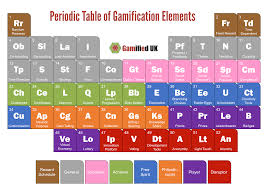
\includegraphics[scale=0.5]{gamification}
        % 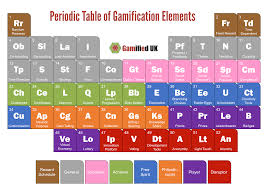
\includegraphics[width=\textwidth]{gamification} bom usar isso quando for artigo em duas colunas, ele pega o tamanho da coluna de texto.
        \caption{Tabela Periódica da Gamificação}
        \label{fig:tabela_periodica}
    \end{figure}
    
    É importante sempre citar as figuras utilizadas no texto através da referência da Figura \ref{fig:tabela_periodica}.
    
    
    Como criar lista? Algumas pessoas deixam nítida a falta de interesse.
    \begin{itemize}
        \item aaa
        \item bbb
        \begin{itemize}
            \item abab
            \item acac
        \end{itemize}
        \item ccc
    \end{itemize}
    
    Também é possível criar listas numeradas utilizando o enumerate, conforme exemplo a seguir.
    
    \begin{enumerate}
        \item aaa
        \item bbb
        \begin{itemize}
            \item abab
            \item acac
        \end{itemize}
        \item ccc
    \end{enumerate}
    


\end{document}
